%%____________________________________________________________________________||

% Overrides original definition
\def\rmhtmet{\mbox{$\mathcal{R}$}\xspace}

\section{Estimation for QCD multijet events \label{sec:qcd}}

One of the major challenges for searches of new physics in the jets +
\met final state is the control of background events from QCD multijet
production. The difficulties in the determination of precise estimates
for this background stem from the large cross sections expected in the
high-energy, high-luminosity hadron collider environment at the LHC,
which are further compounded by the lack of precise theoretical
predictions for the cross sections and kinematic properties of
multijet events. Hence, without special consideration and treatment,
significant uncertainties on large background expectations can
overwhelm any potential sensitivity to new physics signatures.

With regards to QCD multijet production, the approach of this search
is to favour the suppression of the multijet background to a
negligible level over the goal of high efficiency for any given signal
model. A conservative uncertainty on a negligible contribution is
preferred over a procedure that attempts to accurately estimate a
non-negligible contribution from multijet events. The level of
contamination should be sufficiently small (\ie sub-percent level)
such that the associated uncertainty, even if large, will be
sub-dominant with respect to the uncertainties on the remaining SM
backgrounds with genuine \met such as \wj, \znunu, and \ttbar,
henceforth labelled as non-multijet processes.

Any contamination from QCD multijet events is controlled primarily
through the \alphat and \bdphi variables. The \alphat variable is able
to distinguish with high efficiency the sources of ``fake'' \met, such
as jet energy mismeasurement, from those with ``genuine'' \met, such
as neutrinos. The \bdphi variable is also very efficient at
identifying jets that suffer under-measurements, as well as
over-measurements, in (otherwise balanced) multijet events. The
variable is also particularly suited to identifying multijet events
that exhibit significant \met due to the production of neutrinos
(collinear with a jet axis) in semileptonic heavy-flavour decays. Both
variables are individually capable of reducing the yields from
multijet events by several orders of magnitude, and combined provide
an extremely robust method to reject multijet events.

In Fig.~\ref{fig:bDPhi_mhtJetPhi} a comparison of the abilities of the 
\bdphi variable to control the QCD multijet background with a similar 
jet-\mht angular variable \dphimhtj, the minimum azimuthal separation 
between the \mht-vector and the leading four jets, is presented. The 
\bdphi variable exhibits a distribution that is more sharply peaked at 
low values and faster falling than \dphimhtj, providing a better control
of the QCD multijet background. \dphimhtj for QCD conversely has a 
broader distribution with a larger leakage for a comparable azimuthal 
selection. Additionally the \bdphi variable displays robustness in the 
presence of severe event mismeasurement. A mismeasurement is simulated 
by artificially lowering the \pt of the jet that minimises the azimuthal
 separation variable to 41 \GeV and the event variables recomputed. Due 
to the removal of the probe jet from the computation of \bdphi, the 
distribution of angular separation Fig.~\ref{fig:shifted_bDPhi_dist} is 
remains unchanged under severe mismeasurement. The \dphimhtj variable is
 sensitive to such mismeasurement as both \mht and the rank of the 
leading four jets are affected, resulting in a broader distribution with
increased leakage Fig.~\ref{fig:shifted_DPhiMht_dist}.


\begin{figure}[!h]
 \centering
 \subfigure[QCD \bdphi distribution.\label{fig:bDPhi_dist}]{
 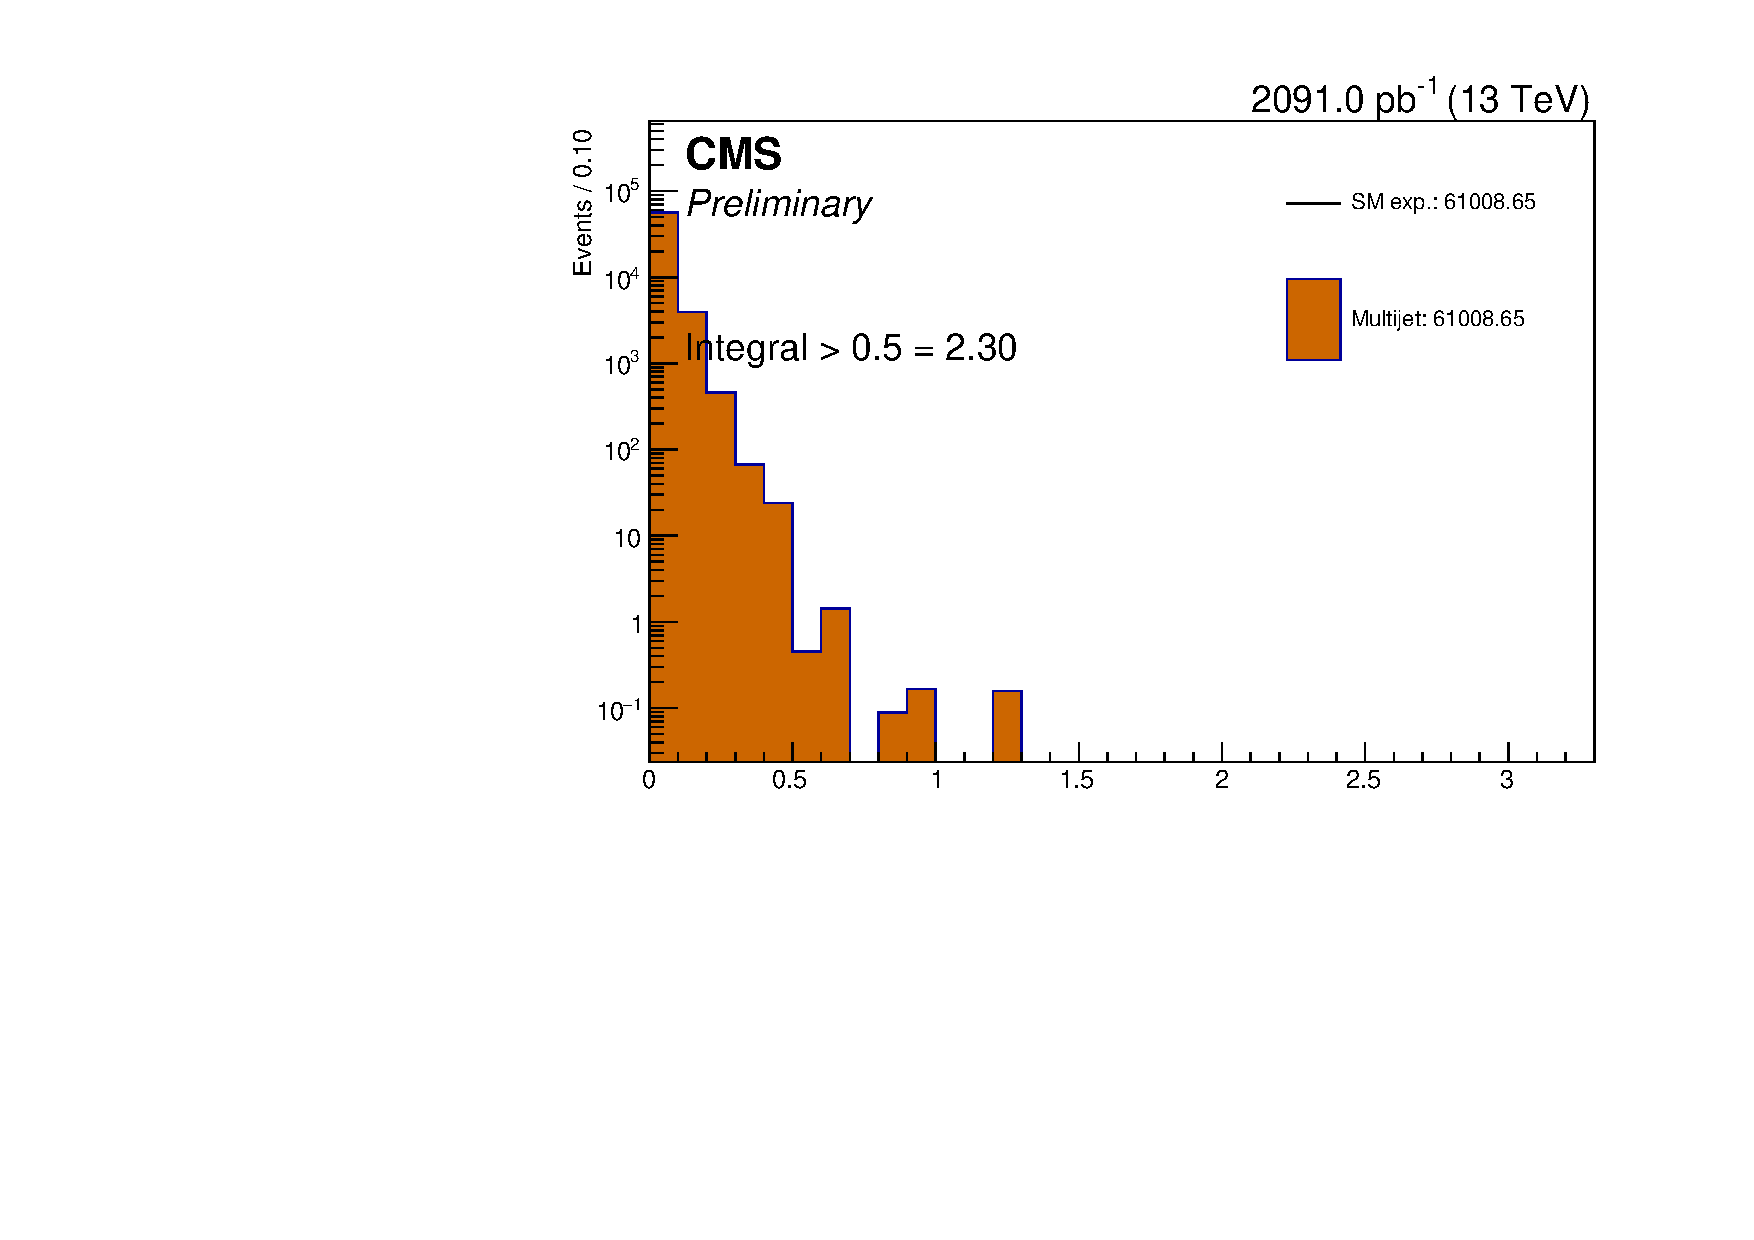
\includegraphics[width=0.5\textwidth]{figures/qcd/v6/bDPhi/biasedDPhi_all_800}
 }
 \subfigure[QCD \dphimhtj distribution.\label{fig:DPhiMht_dist}]{
 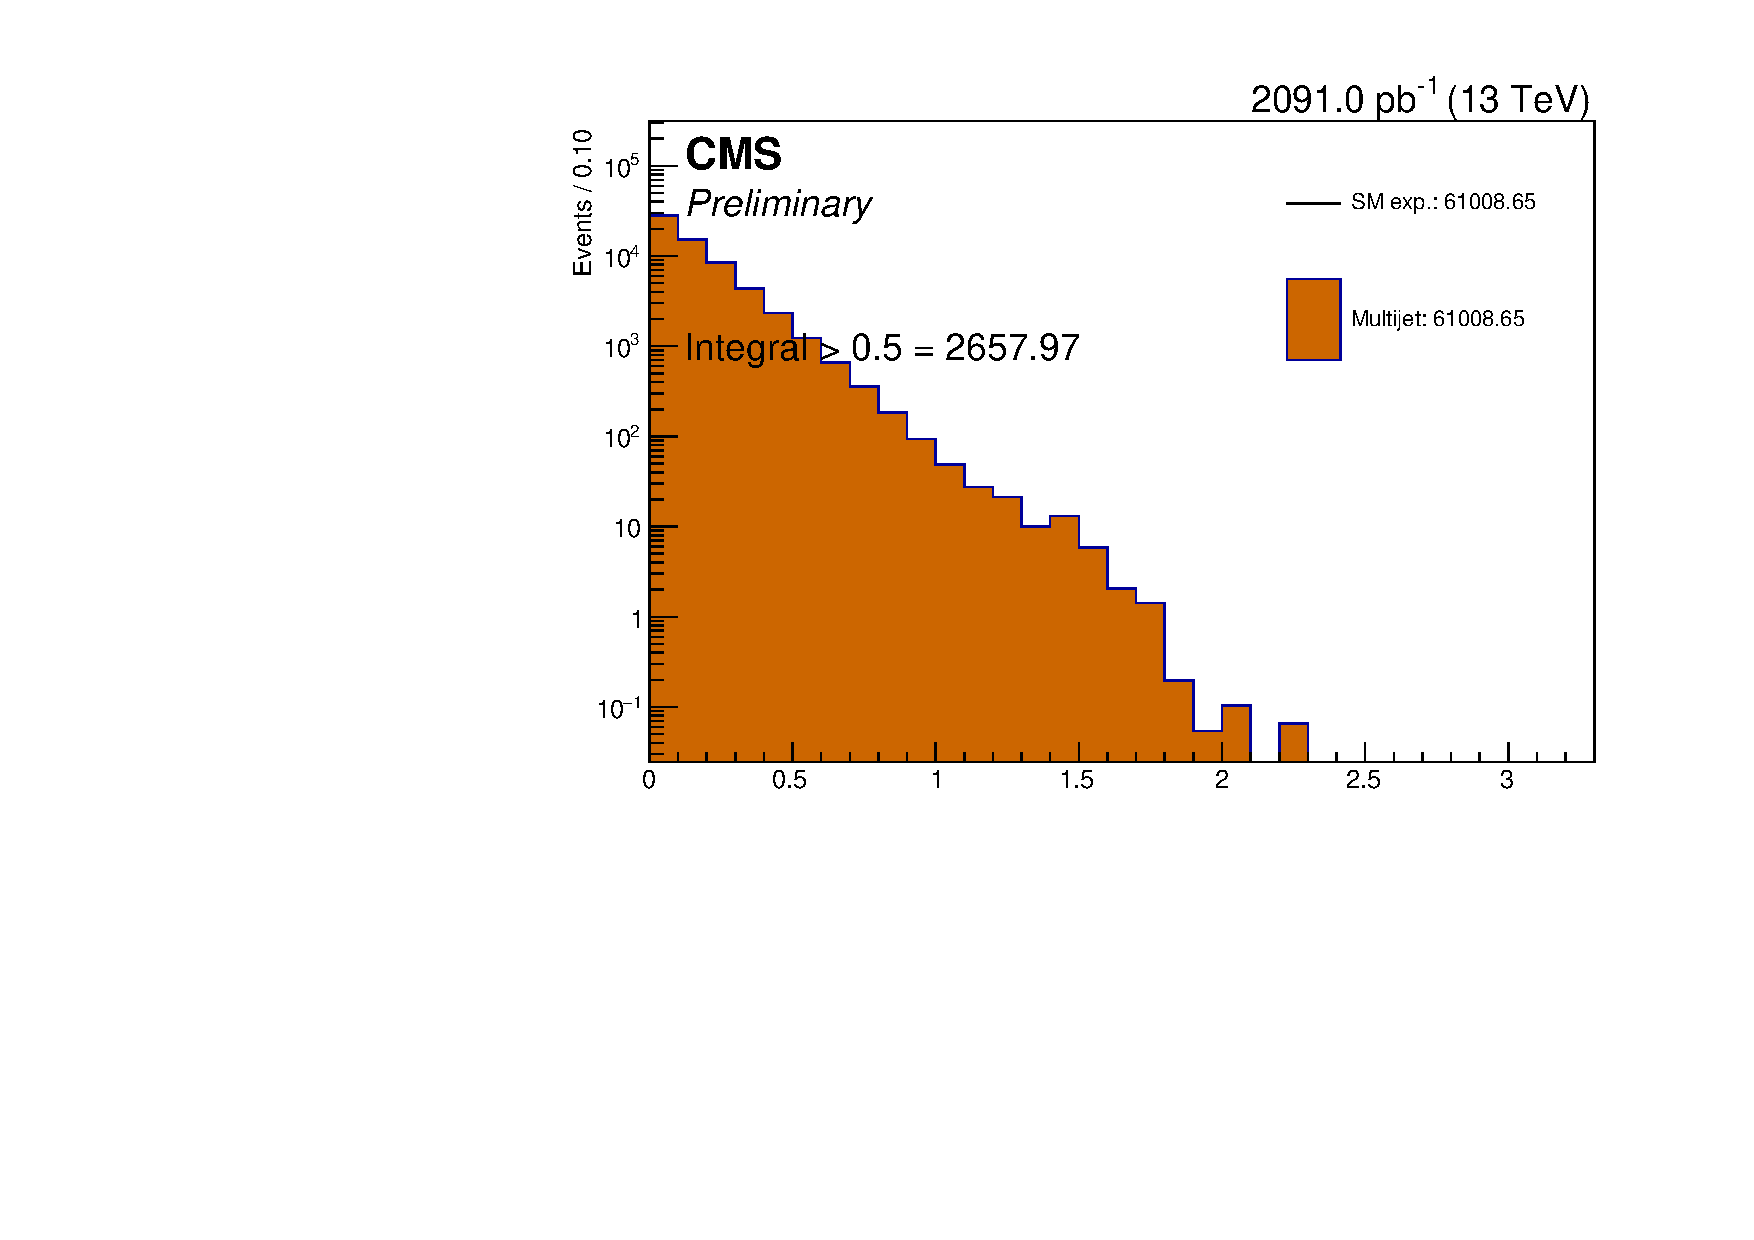
\includegraphics[width=0.5\textwidth]{figures/qcd/v6/bDPhi/minDeltaPhiMht_all_800}
 } \\
 \subfigure[QCD \bdphi distribution with mismeasurement.\label{fig:shifted_bDPhi_dist}]{
 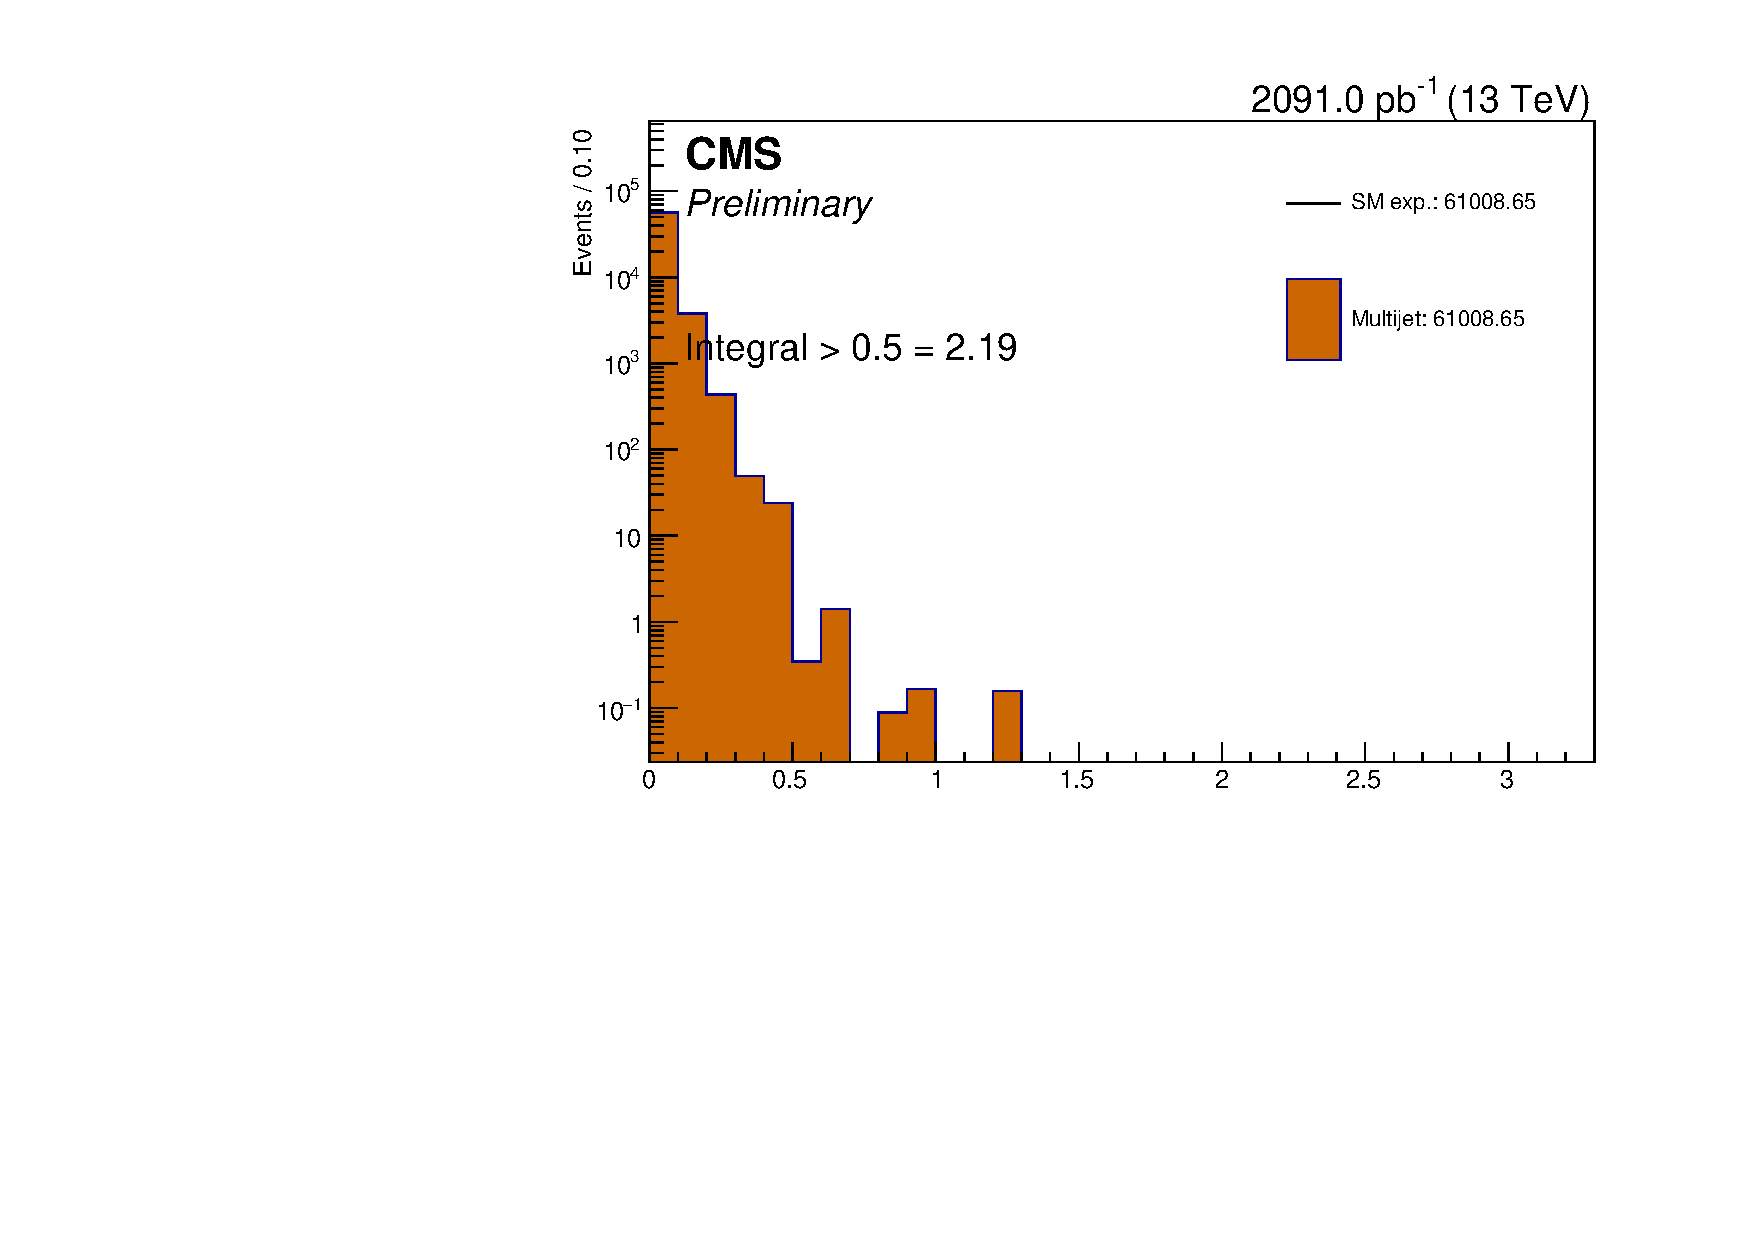
\includegraphics[width=0.5\textwidth]{figures/qcd/v6/bDPhi/shiftedMinBDPhi_all_800}
 }
 \subfigure[QCD \dphimhtj distribution with mismeasurement.\label{fig:shifted_DPhiMht_dist}]{
 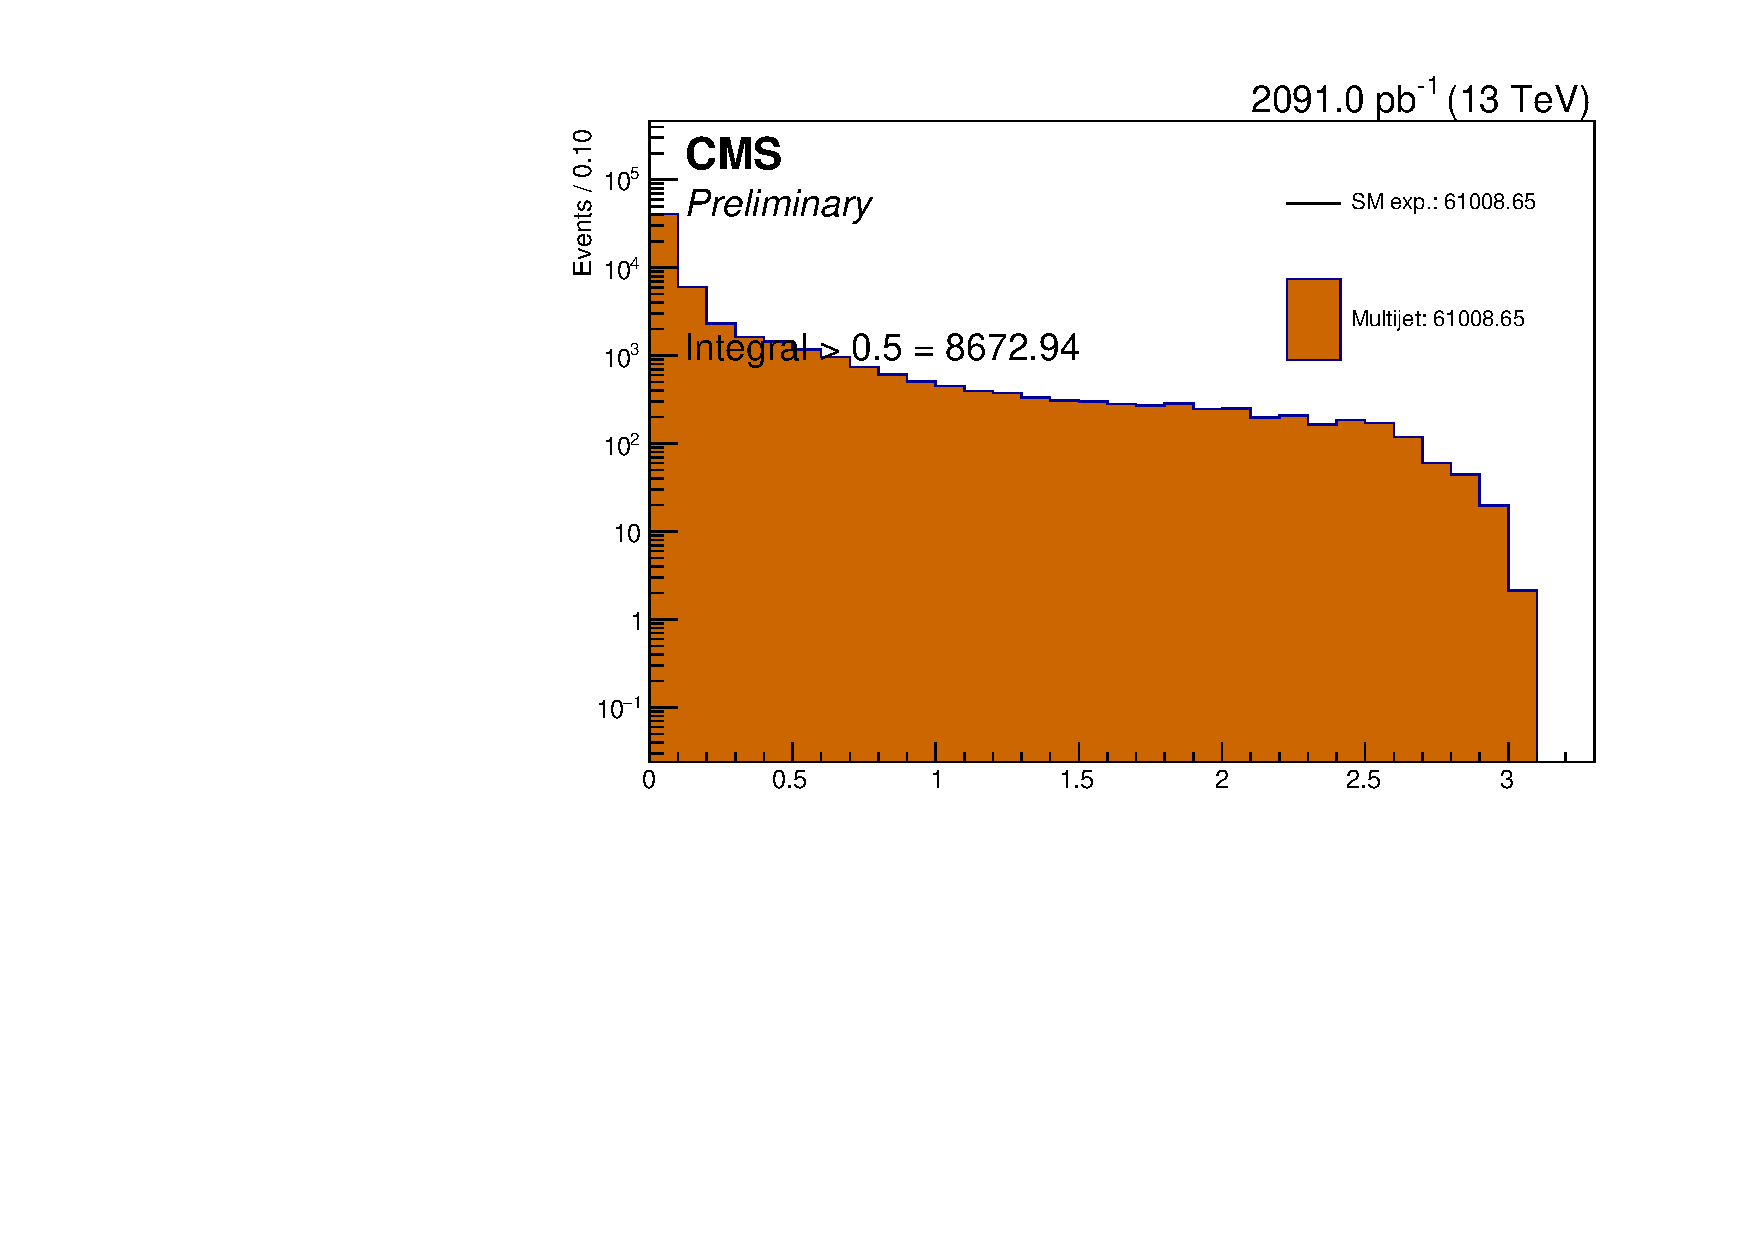
\includegraphics[width=0.5\textwidth]{figures/qcd/v6/bDPhi/shiftedMinDeltaPhiMht_all_800}
 } \\
 \caption{\bdphi and \dphimhtj distributions of QCD multijet simulation
 after analysis selections for \scalht $> 800$ \GeV in the case of
 nominal reconstruction (a), (b) and severe mismeasurement (c), (d). The
 total number of events that pass a $\Delta\phi > 0.5$ selection of the
 respective quantity are indicated. }
 \label{fig:bDPhi_mhtJetPhi}
\end{figure}


In Run~1, the \alphat and \bdphi thresholds required to control
multijet contamination to the required level were determined by a
dedicated data-driven method, which relied on multijet-enriched
sidebands in the variables \alphat, \bdphi, and \mhtmet. The \mhtmet
variable, discussed in Sec.~\ref{sec:selection}, is used to filter QCD
multijet events that contain soft jets below threshold contributing
significantly to \mht. The method relied on extrapolating the
exponential modelling of the number of multijet events passing and
failing a requirement on the variable \mhtmet, \ie the pass/fail ratio
\rmhtmet, as a function of \alphat for a given signal region bin
(defined in terms of \njet, \nb, and \scalht). In essence, the
approach employed was an ABCD method that accounted for the
correlation between the variables \rmhtmet and \alphat, followed
by an additional requirement on \bdphi determined and validated in a
data control sideband.

For this search, we employ a simpler approach that relies on the
determination of the ratio \rmhtmet per (\njet,\scalht) bin from
simulation. The ratio is determined following the application of the
\alphat and \bdphi requirements, which in the former case are
\scalht-dependent. For the region $\scalht > 800\gev$, the requirement
$\mht > 130\gev$ is made in place of any on \alphat. No \alphat nor
\mht requirements are imposed for events in the monojet
category.\footnote{For events in the monojet bin, an implicit
  requirement of $\mht > 200\gev$ is indeed made given that $\mht =
  \scalht$ for monojet events. No \alphat calculation can be made
  given the absence of a second jet.} The requirements on \alphat,
\mht, and \bdphi as a function of \scalht are summarised in
Sec.~\ref{sec:selection}. Each ratio \rmhtmet is then used as a
multiplier on data counts per (\njet,\scalht) bin obtained in the
\mhtmet data sideband. The data counts are corrected for contributions
from V+jets and \ttbar (and other residual contributions from
non-multijet processes) in order to obtain an estimate of the number
of QCD multijet events, $\mathcal{Q}$ in each sideband bin. The
product of these (corrected) counts and the ratio, $\mathcal{Q} \times
r\mhtmet$, provides an estimate of the level of QCD multijet events in
each (\njet,\scalht) bin of the signal region. The estimate is
currently made inclusively with respect to the \nb\ and \mht for each
(\njet,\scalht) bin. The method is outlined in more detail below.

\begin{figure}[!h]
  \centering
  \subfigure[QCD events in signal region.\label{fig:qcd_pass}]{
    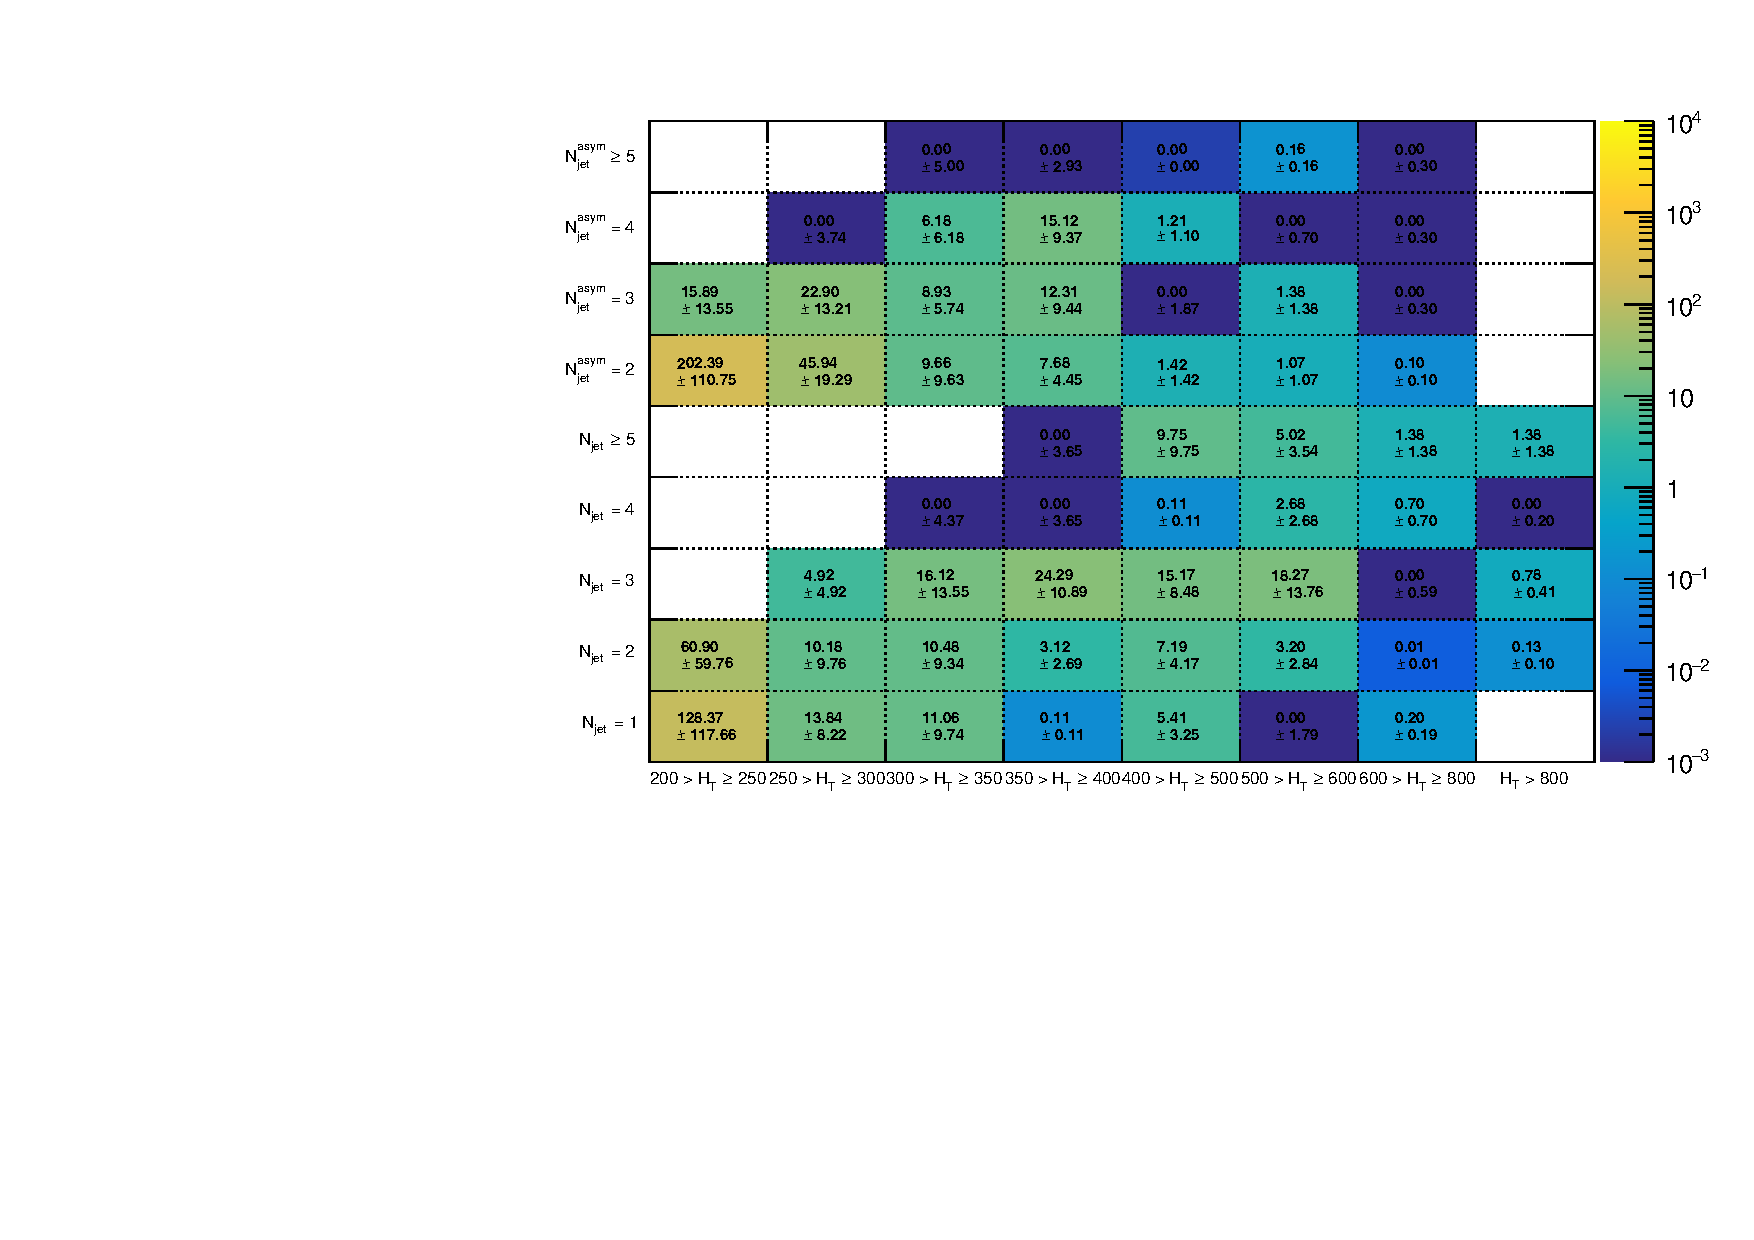
\includegraphics[width=0.5\textwidth]{figures/qcd/v6/QCD/SigTrig_PassMoM_NJet_vs_HT_bDPhigt0p5_Log}
  } 
  \subfigure[QCD events in \mhtmet sideband.\label{fig:qcd_fail}]{
    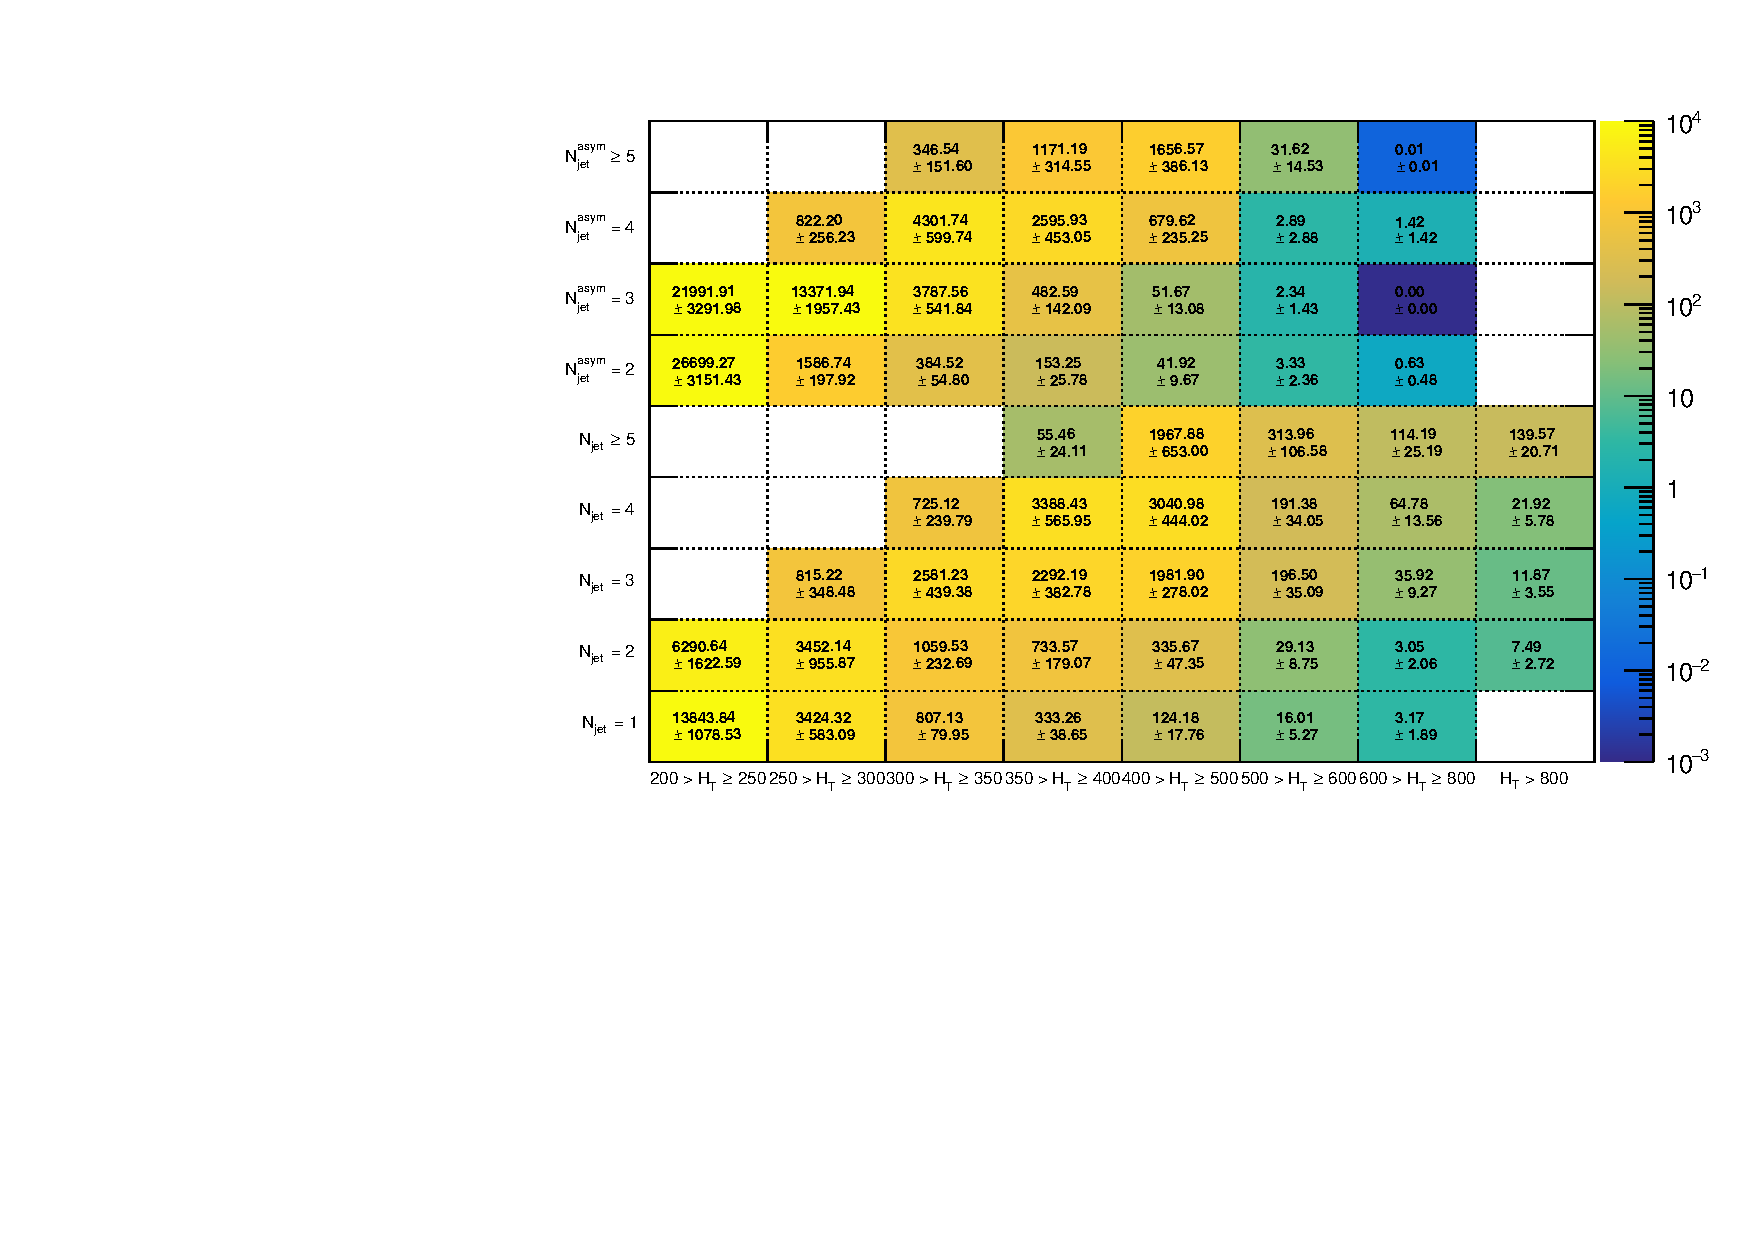
\includegraphics[width=0.5\textwidth]{figures/qcd/v6/QCD/SigTrig_FailMoM_NJet_vs_HT_bDPhigt0p5_Log}
  } \\
  \subfigure[Ratio \rmhtmet for QCD events.\label{fig:qcd_ratio}]{
    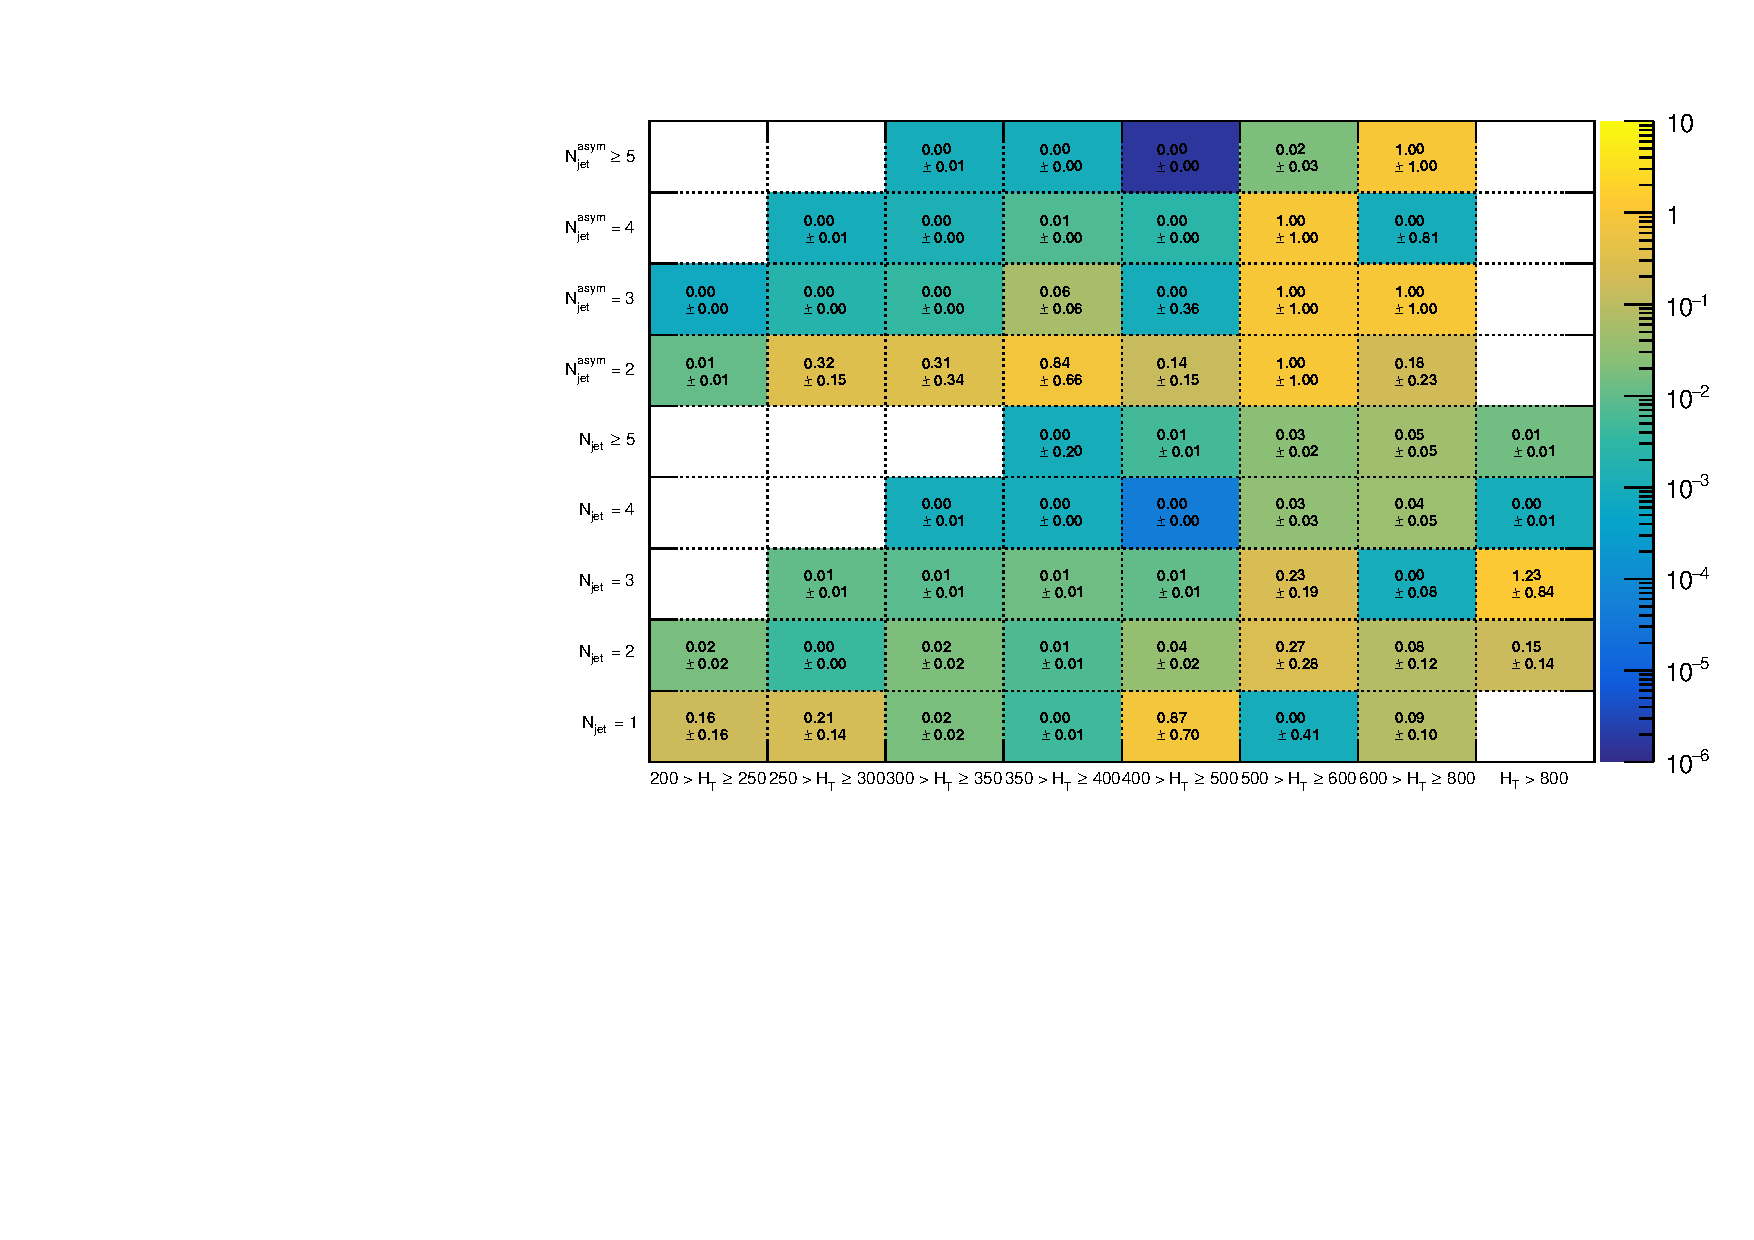
\includegraphics[width=0.5\textwidth]{figures/qcd/v6/QCD/SigTrig_RMoM_NJet_vs_HT_bDPhigt0p5_Log}
  } 
  \subfigure[EWK events in \mhtmet sideband.\label{fig:ewk_fail}]{
    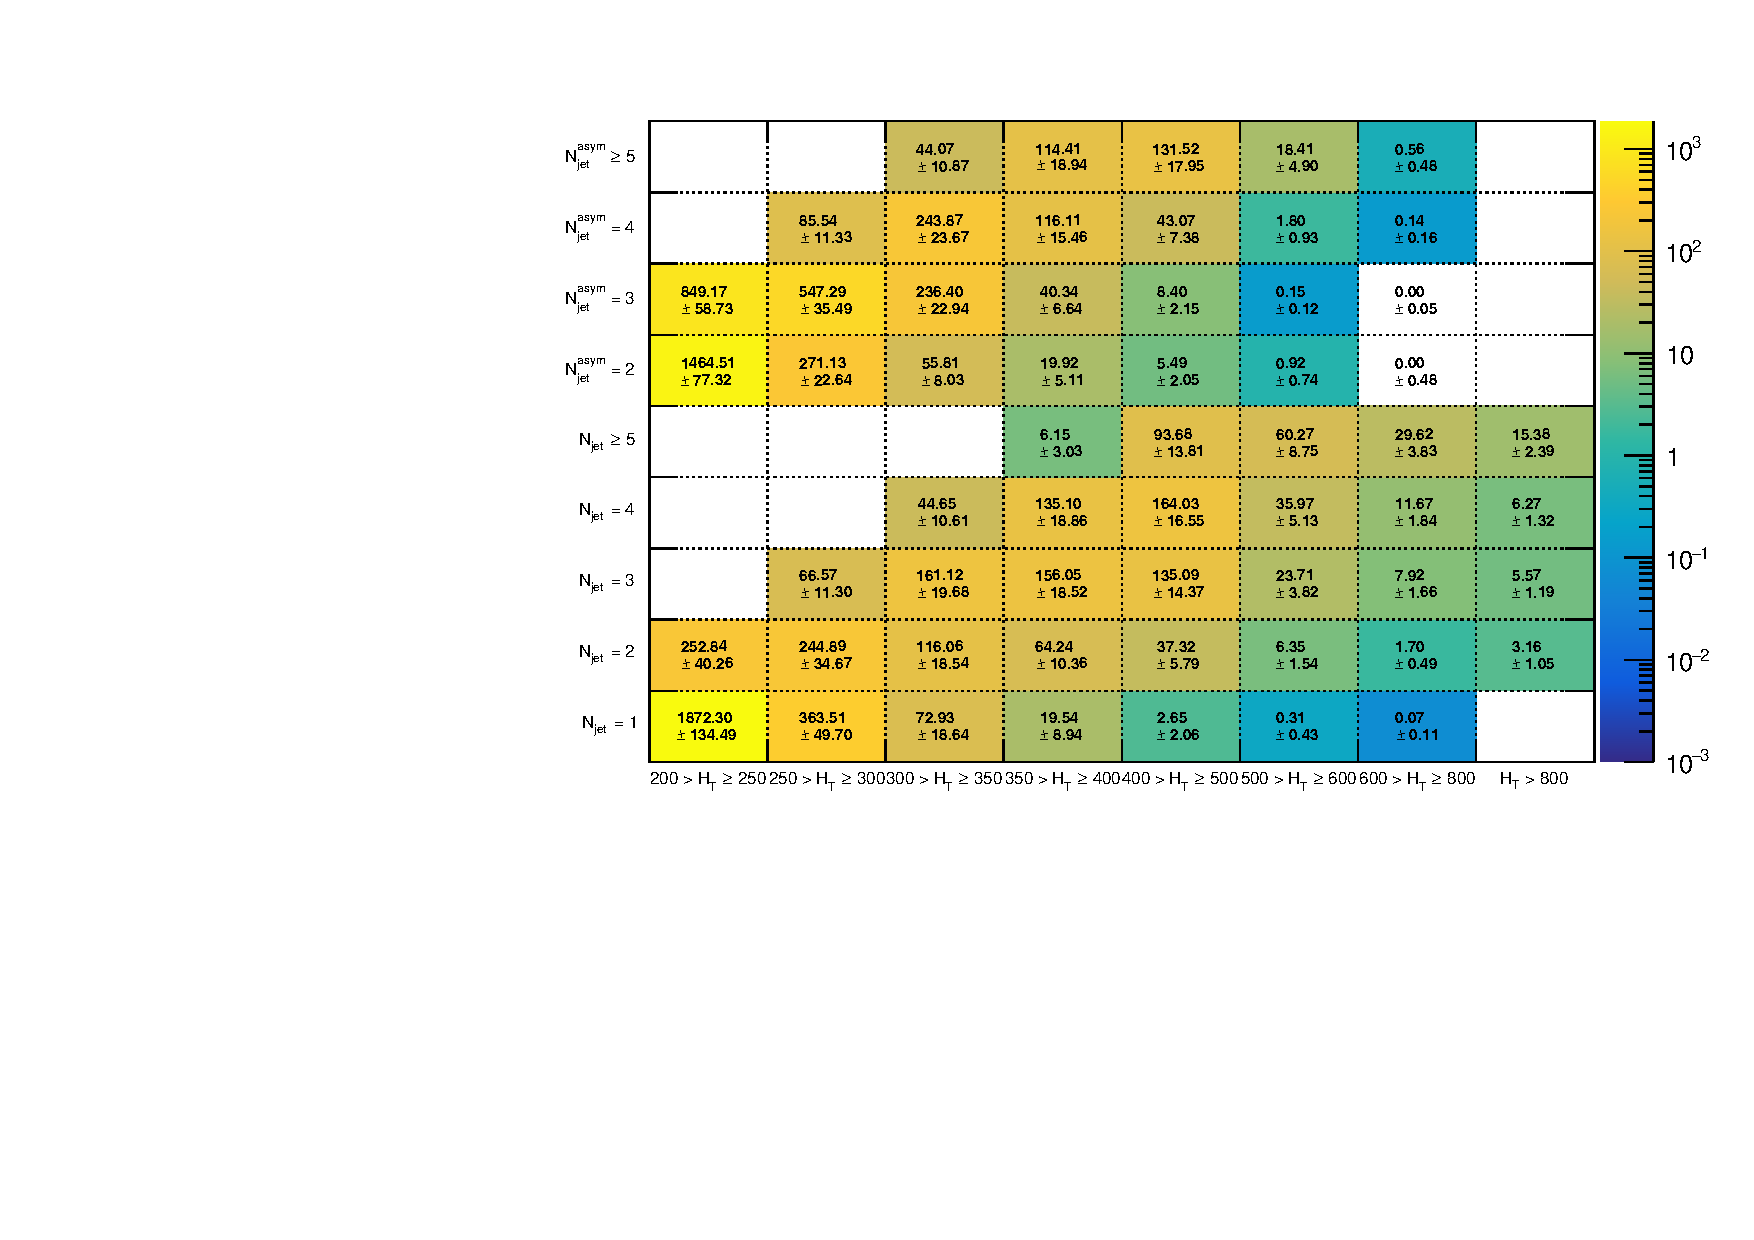
\includegraphics[width=0.5\textwidth]{figures/qcd/v6/Ewk/EwkPred_SigTrig_FailMoM_NJet_vs_HT_bDPhigt0p5_Log}
   %    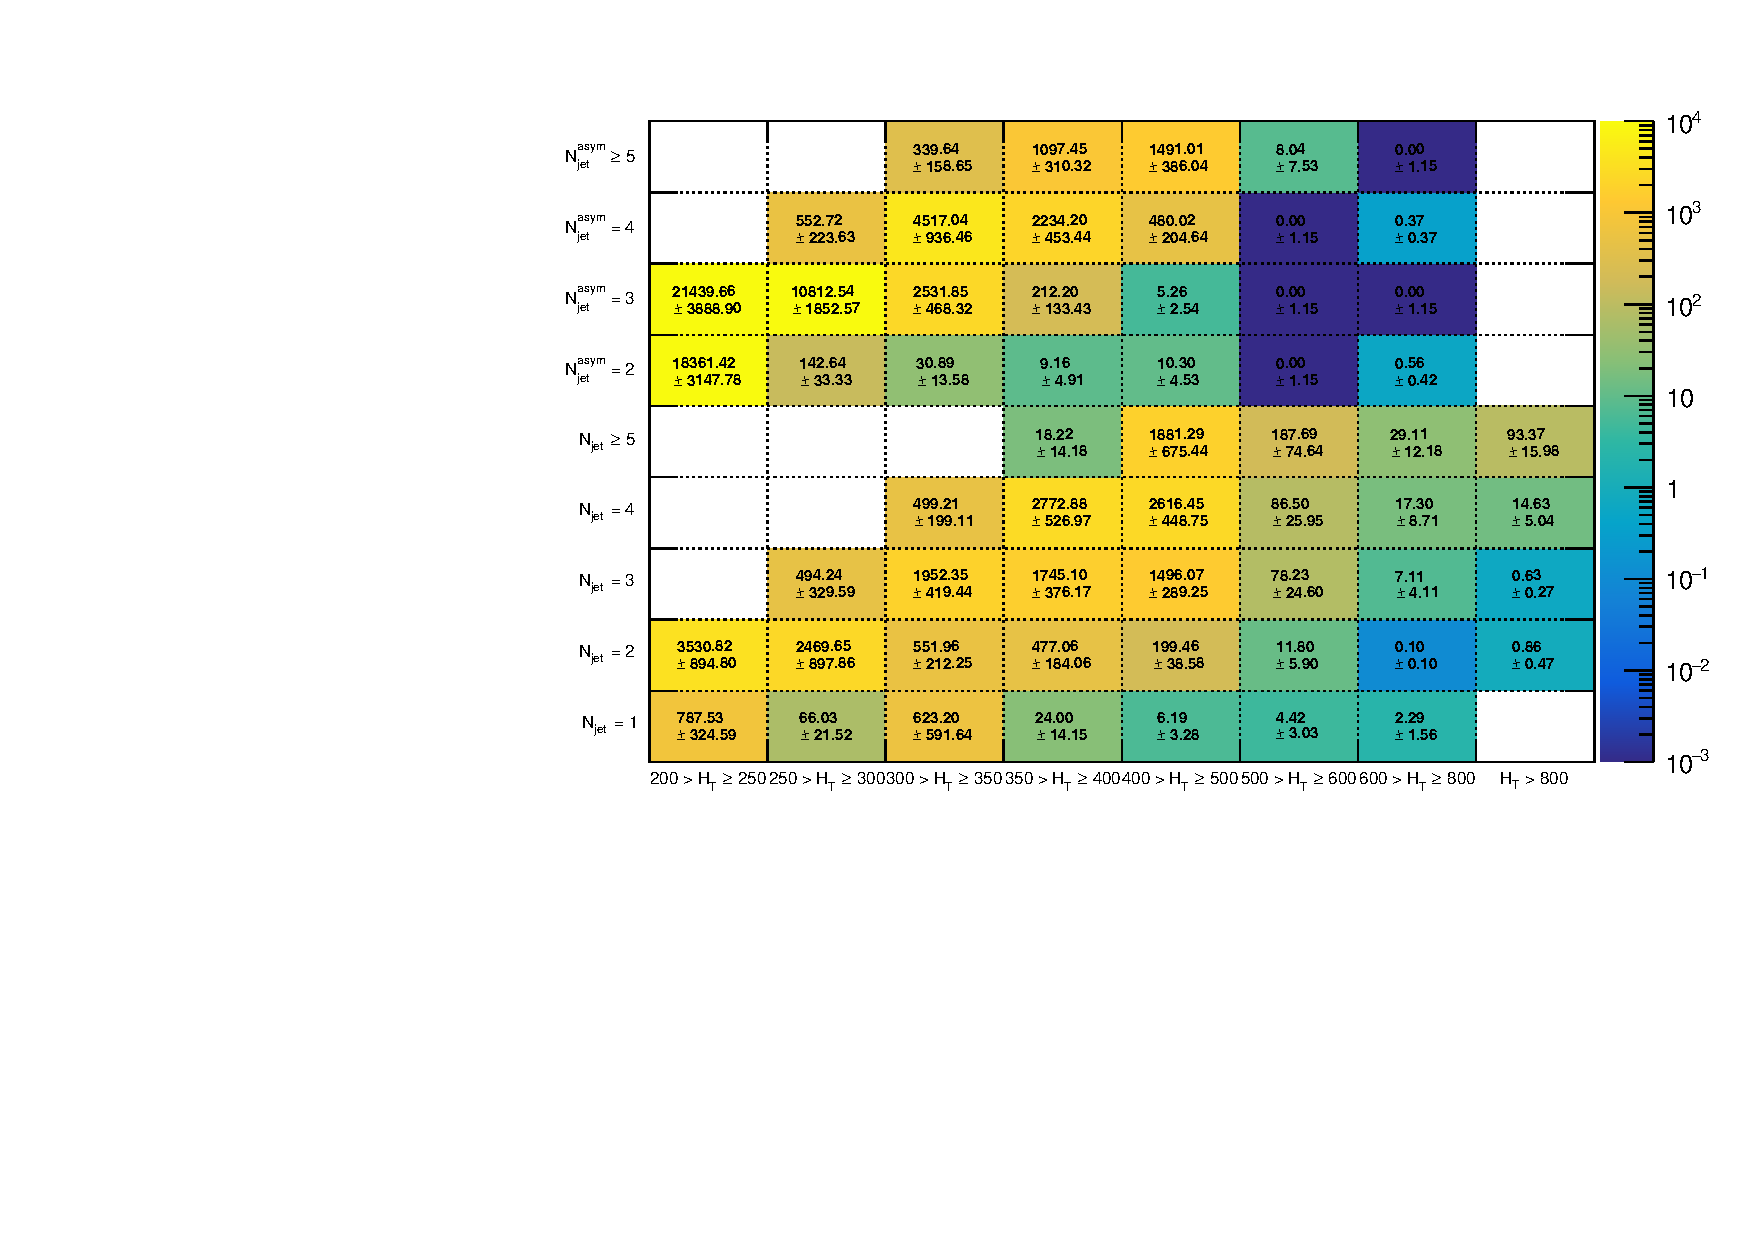
\includegraphics[width=0.5\textwidth]{figures/qcd/v6/Ewk/SigTrig_FailMoM_NJet_vs_HT_bDPhigt0p5_Log}
  } \\
  \caption{Expected number of QCD multijet events determined from
    simulation, binned according to \njet and \scalht, that (a) satisfy
    and (b) fail the requirement $\mhtmet < 1.25$. Also shown in (c)
    is the ratio \rmhtmet for QCD multijets, again determined from
    simulation. Finally, (d) shows the expected number of EWK events
    (V+jets and \ttbar, plus other residual non-multijet backgrounds)
    that fail the $\mhtmet < 1.25$ requirement, again determined from
    simulation and binned according to \njet and \scalht.}
  \label{fig:qcd_plots}
\end{figure}

The number of counts from multijet events satisfying and failing the
requirement $\mhtmet < 1.25$, \ie the pass/fail ratio \rmhtmet, is
determined from simulation per (\njet,\scalht) bin. The pass and fail
counts and the ratios are summarised in Fig.~\ref{fig:qcd_pass},
\ref{fig:qcd_fail}, and \ref{fig:qcd_ratio}. Figure~\ref{fig:ewk_fail}
shows the expected counts from non-multijet backgrounds in the \mhtmet
sideband, as determined from simulation.

\begin{figure}[!h]
  \centering
  \subfigure[Binned data counts in \mhtmet sideband.\label{fig:data_fail}]{
    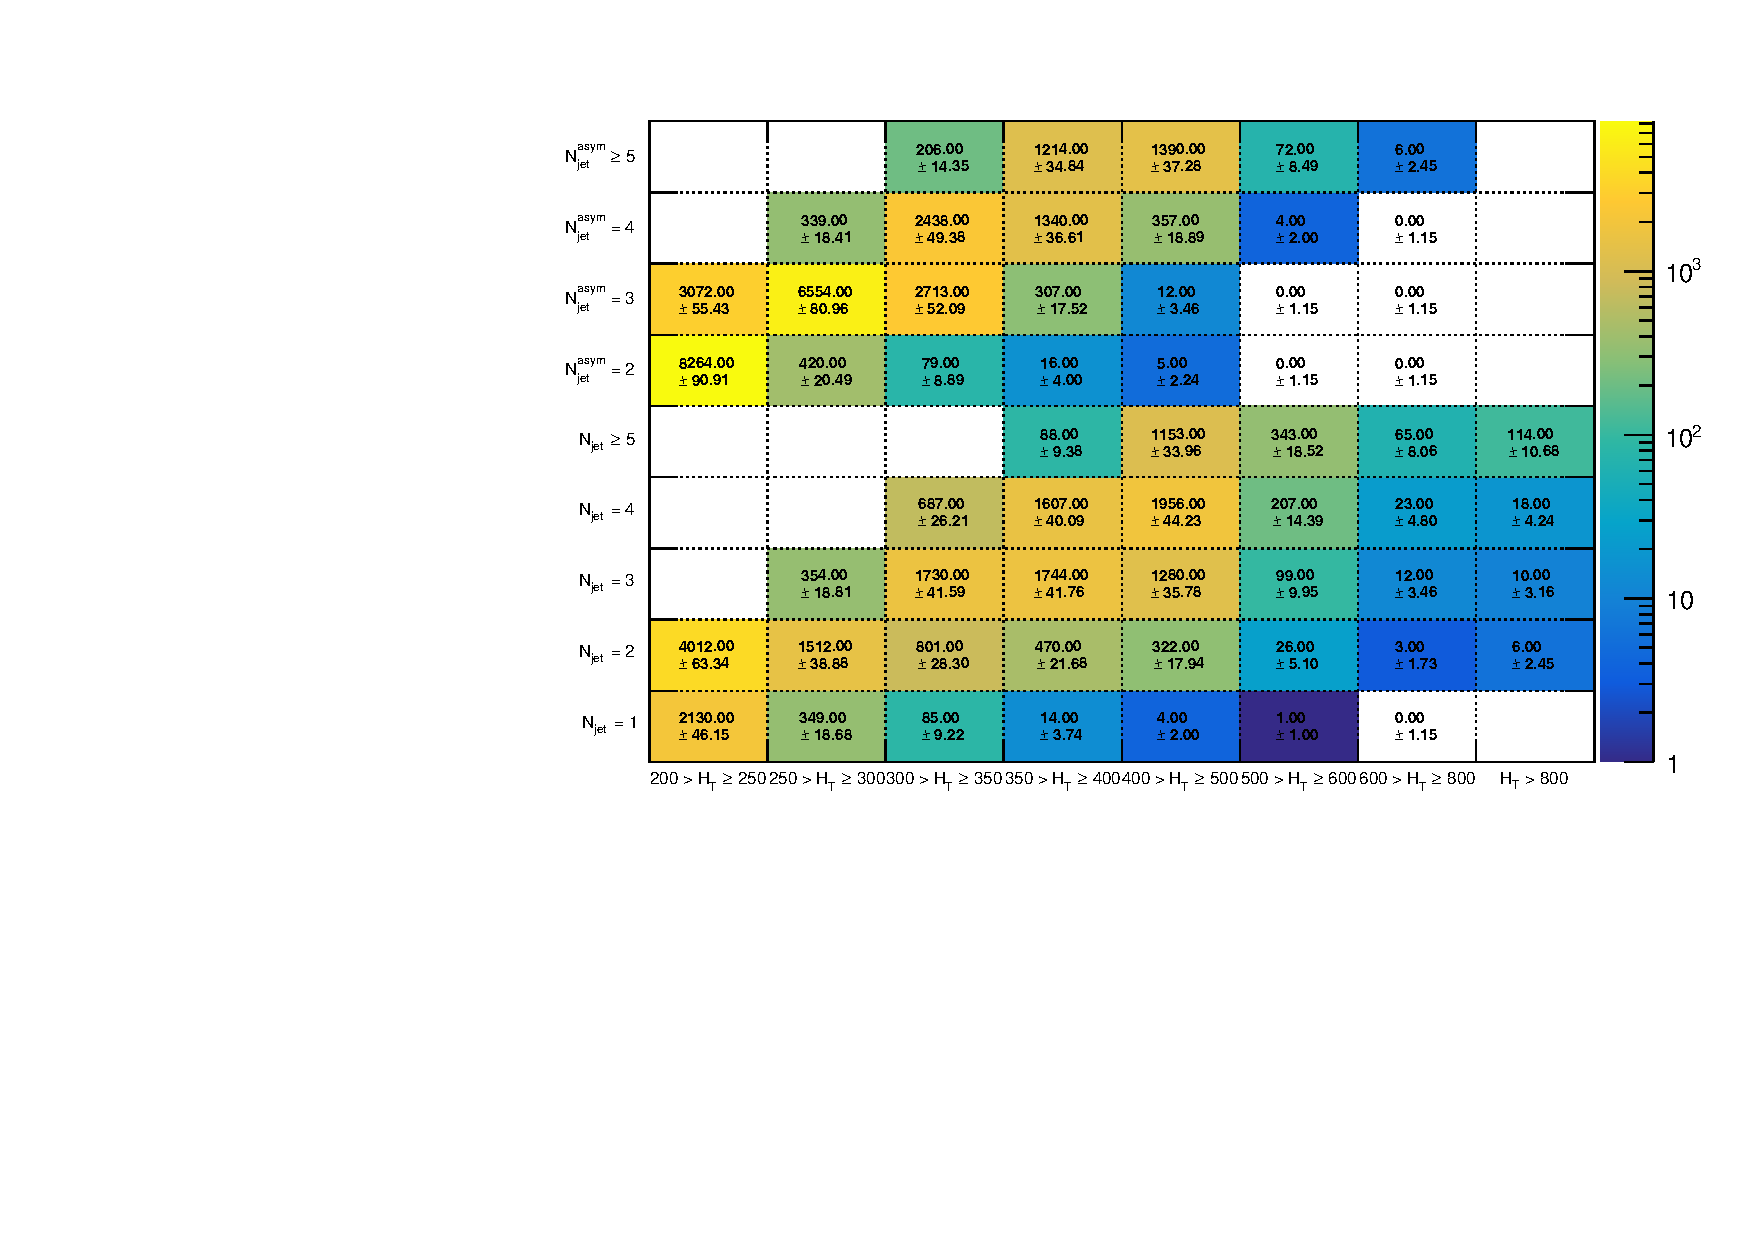
\includegraphics[width=0.5\textwidth]{figures/qcd/v6/SigTrig_FailMoM_NJet_vs_HT_bDPhigt0p5_Log}
  } 
  \subfigure[Corrected data counts in \mhtmet sideband.\label{fig:data_corr}]{
    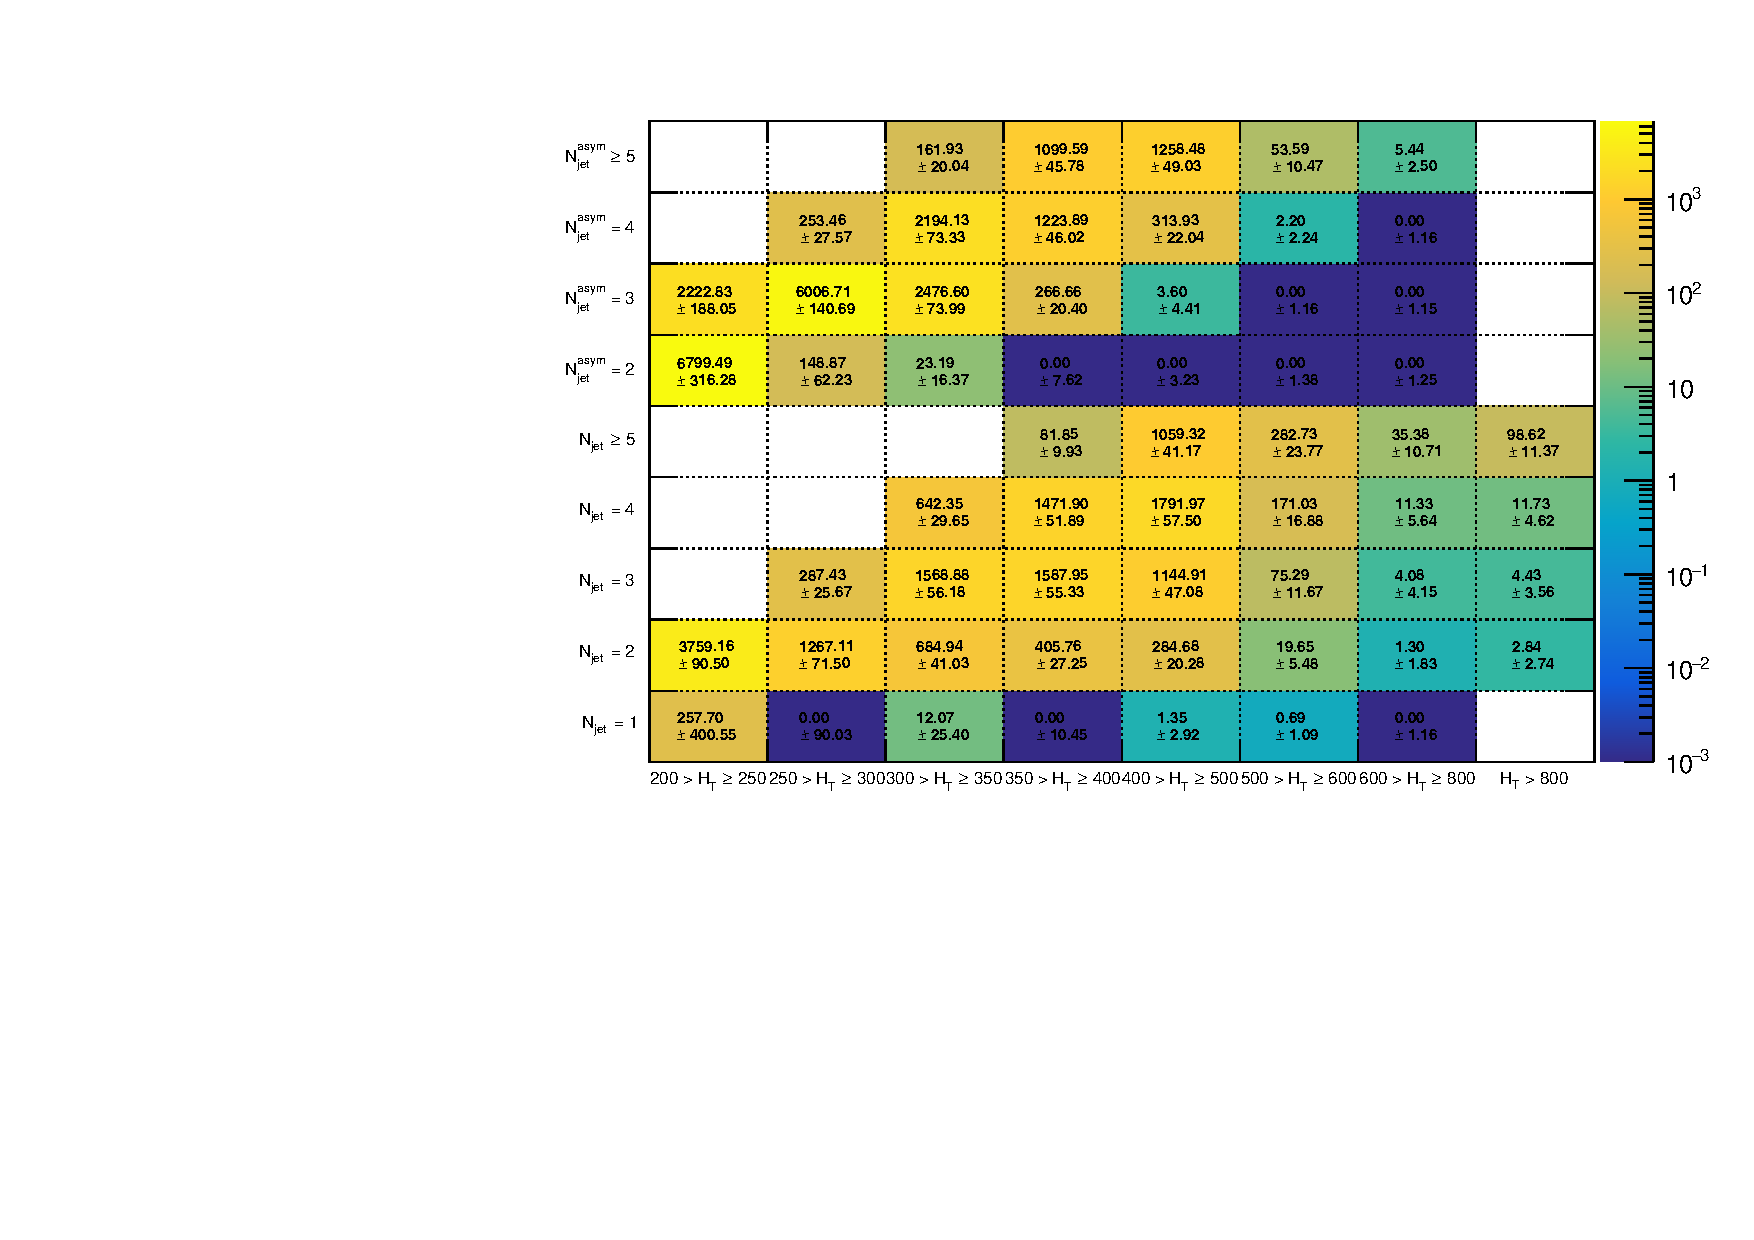
\includegraphics[width=0.5\textwidth]{figures/qcd/v6/DataNoEwk_SigTrig_FailMoM_NJet_vs_HT_bDPhigt0p5_Log}
  } \\
  \subfigure[QCD multijet predictions in the signal region.\label{fig:qcd_pred}]{
    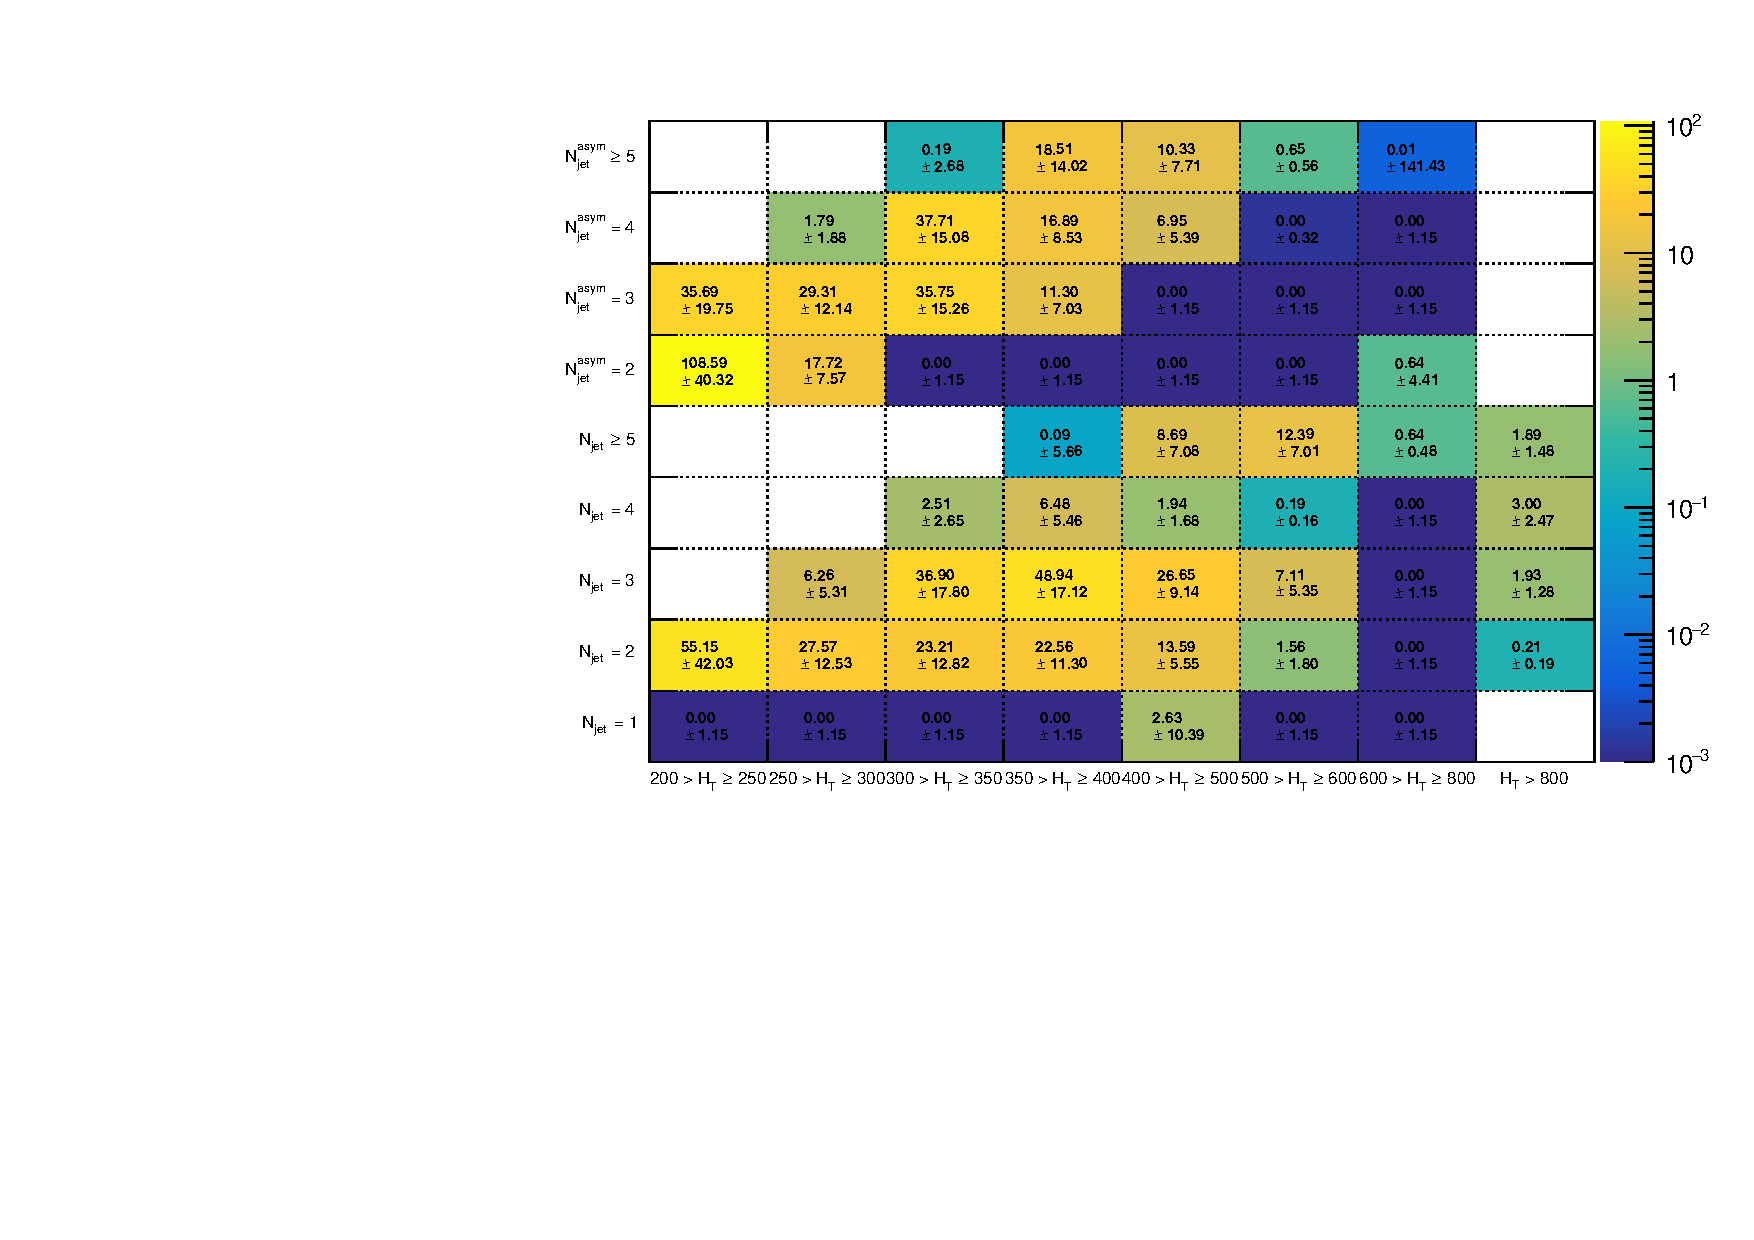
\includegraphics[width=0.5\textwidth]{figures/qcd/v6/DataNoEwk_SigTrig_QCDPred_NJet_vs_HT_bDPhigt0p5_Log}
  } 
  \subfigure[Ratio of predicted multijet and non-multijet yields.\label{fig:qcd_ewk_ratio}]{
    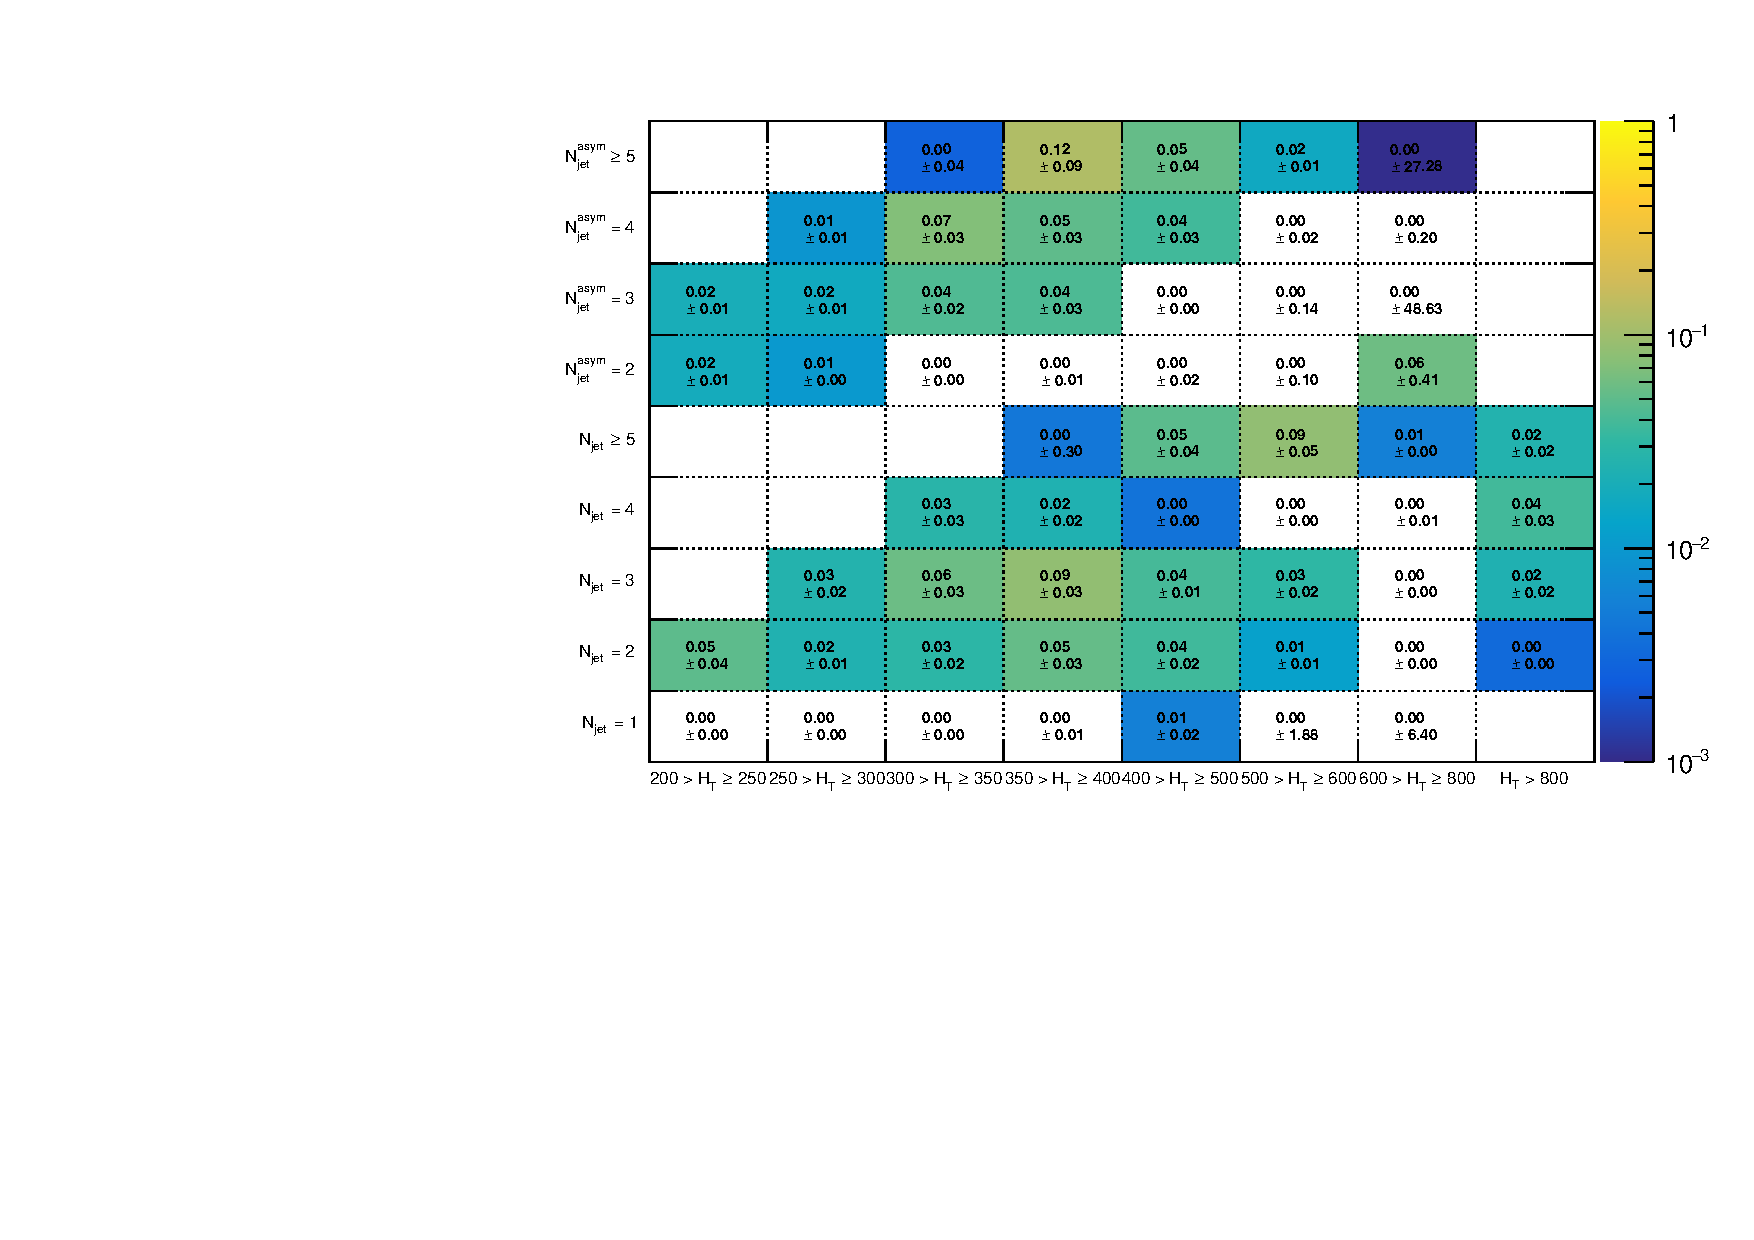
\includegraphics[width=0.5\textwidth]{figures/qcd/v6/DataNoEwk_SigTrig_QCDPredDivEwk_NJet_vs_HT_bDPhigt0p5_Log}
  } \\
  \caption{Expected number of QCD multijet events determined from
    simulation, binned according to \njet and \scalht that (a) fail
    and (b) satisfy the $\mhtmet < 1.25$ requirement. Also shown in
    (c) is the ratio \rmhtmet for QCD multijets, again determined from
    simulation. Finally, (d) shows the expected number of EWK events
    (V+jets and \ttbar plus other residual non-multijet backgrounds)
    that the fail the $\mhtmet < 1.25$ requirement, again determined
    from simulation and binned according to \njet and \scalht.}
  \label{fig:qcd_plots2}
\end{figure}

The data counts in the \mhtmet sideband are collected with the
\verb!HLT_HTxxx_AlphaT0pyy!  and \verb!HLT_HT800! signal triggers
described in Sec.~\ref{sec:triggers}. Events satisfy the full signal
region requirements plus the inverted \mhtmet requirement and are
binned according to \njet and \scalht. Any contribution from
non-multijet backgrounds (V+jets, \ttbar, \etc) in each bin is
estimated from simulation\footnote{In the future, the counts from
  non-multijet backgrounds will be estimated from the muon data
  control samples and transfer factors determined from simulation
  (using the method described in Sec.~\ref{sec:backgroundmet}).} and
subtracted from the data counts. Any remaining counts, $\mathcal{Q}$,
are assumed to arise from multijet production.
Figure~\ref{fig:data_fail} shows the observed counts in the \mhtmet
sideband, and Fig.~\ref{fig:data_corr} shows the counts after
subtracting the expected contributions from non-multijet processes.
Figure~\ref{fig:qcd_pred} shows the predicted counts for the multijet
contribution in the signal region bins, which are obtained from the
products of \rmhtmet and $\mathcal{Q}$, summarised in
Figs.~\ref{fig:qcd_ratio} and \ref{fig:data_corr}. Finally,
Fig.~\ref{fig:qcd_ewk_ratio} shows the ratios of predicted multijet
counts with respect to the expected EWK counts, in order to quantify
the (predicted) relative contamination from multijet events in the
signal region bins. \mht and \nb shapes derived from simulation are used to predict the distribution 
of QCD events, which are validated by data-driven methods as shown in App.~\ref{app:qcdPredictionValidation}. 
No significant difference in shape is observed between Monte Carlo and data predictions, 
with QCD and EWK are compatible within the quoted statistical and systematic uncertainties.



%% The predictions summarised in Fig.~\ref{fig:qcd_ewk_ratio} support the
%% expectation based on experience with 8~TeV data that the \HT-dependent
%% \alphat thresholds defined in Table~\ref{tab:sr-selections} and the
%% requirement of $\bdphi > 0.5$ are sufficient to reduce the multijet
%% contamination in all bins of the signal region to the sub-percent with
%% respect to the total non-multijet background. With this level of
%% suppression, it is expected that the uncertainty associated with the
%% residual multijet contamination to be sub-dominant with respect to,
%% and fully absorbed by, the systematic uncertainties on the non-multijet
%% backgrounds, which are expected to be at the level of $\sim$10\% or
%% larger. 

The predictions summarised in Fig.~\ref{fig:qcd_ewk_ratio} show that 
the \HT-dependent \alphat thresholds defined in Table~\ref{tab:sr-selections} 
and the requirement of $\bdphi > 0.5$ suppress the multijet
contamination in all bins of the signal region to percent-level or smaller with
respect to the total non-multijet background. These predicted multijet events are 
included as a background contribution to the likelihood model.
